%\subsection{Portfolio f\"ur Industry Paper und Evaluation Methods (Gr\"o\ss{}e entspricht der Anzahl)}
%\begin{figure}
\begin{center}
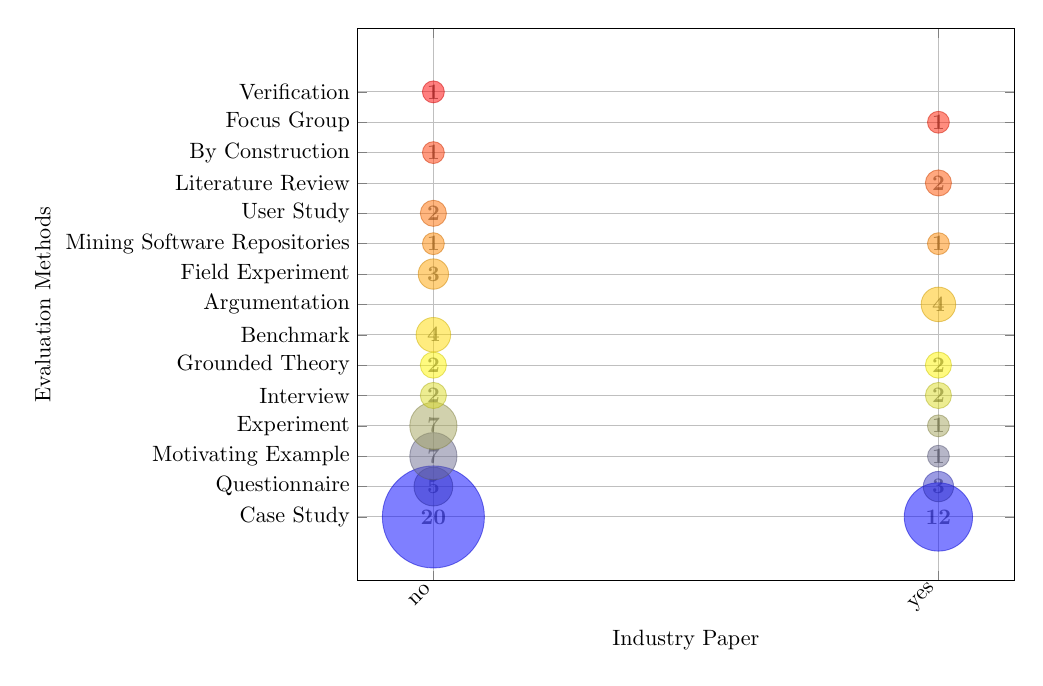
\begin{tikzpicture}[scale=.8]
\begin{axis}[scatter,
    width=.99\linewidth,
    cycle multi list=Spectral,
    every axis plot/.append style={draw, fill, fill opacity=0.5},
    scatter src=y,
    nodes near coords style={color=black,font=\small},
    enlargelimits=0.15,
    x tick label style={rotate=45,anchor=east},
    xtick={0,1}, xticklabels={no,yes},
    xlabel={Industry Paper},
    ytick={0,1,2,3,4,5,6,7,8,9,10,11,12,13,14}, yticklabels={Case Study,Questionnaire,Motivating Example,Experiment,Interview,Grounded Theory,Benchmark,Argumentation,Field Experiment,Mining Software Repositories,User Study,Literature Review,By Construction,Focus Group,Verification},
    ylabel={Evaluation Methods},
    grid=both
]

\addplot[mark size=23.048,opacity=0.5,text=black] coordinates { (0,0) } node[text=black,font=\bfseries] {20};
\addplot[mark size=8.762,opacity=0.5,text=black] coordinates { (0,1) } node[text=black,font=\bfseries] {5};
\addplot[mark size=10.667,opacity=0.5,text=black] coordinates { (0,2) } node[text=black,font=\bfseries] {7};
\addplot[mark size=10.667,opacity=0.5,text=black] coordinates { (0,3) } node[text=black,font=\bfseries] {7};
\addplot[mark size=5.905,opacity=0.5,text=black] coordinates { (0,4) } node[text=black,font=\bfseries] {2};
\addplot[mark size=5.905,opacity=0.5,text=black] coordinates { (0,5) } node[text=black,font=\bfseries] {2};
\addplot[mark size=7.810,opacity=0.5,text=black] coordinates { (0,6) } node[text=black,font=\bfseries] {4};
\addplot[mark size=6.857,opacity=0.5,text=black] coordinates { (0,8) } node[text=black,font=\bfseries] {3};
\addplot[mark size=4.952,opacity=0.5,text=black] coordinates { (0,9) } node[text=black,font=\bfseries] {1};
\addplot[mark size=5.905,opacity=0.5,text=black] coordinates { (0,10) } node[text=black,font=\bfseries] {2};
\addplot[mark size=4.952,opacity=0.5,text=black] coordinates { (0,12) } node[text=black,font=\bfseries] {1};
\addplot[mark size=4.952,opacity=0.5,text=black] coordinates { (0,14) } node[text=black,font=\bfseries] {1};
\addplot[mark size=15.429,opacity=0.5,text=black] coordinates { (1,0) } node[text=black,font=\bfseries] {12};
\addplot[mark size=6.857,opacity=0.5,text=black] coordinates { (1,1) } node[text=black,font=\bfseries] {3};
\addplot[mark size=4.952,opacity=0.5,text=black] coordinates { (1,2) } node[text=black,font=\bfseries] {1};
\addplot[mark size=4.952,opacity=0.5,text=black] coordinates { (1,3) } node[text=black,font=\bfseries] {1};
\addplot[mark size=5.905,opacity=0.5,text=black] coordinates { (1,4) } node[text=black,font=\bfseries] {2};
\addplot[mark size=5.905,opacity=0.5,text=black] coordinates { (1,5) } node[text=black,font=\bfseries] {2};
\addplot[mark size=7.810,opacity=0.5,text=black] coordinates { (1,7) } node[text=black,font=\bfseries] {4};
\addplot[mark size=4.952,opacity=0.5,text=black] coordinates { (1,9) } node[text=black,font=\bfseries] {1};
\addplot[mark size=5.905,opacity=0.5,text=black] coordinates { (1,11) } node[text=black,font=\bfseries] {2};
\addplot[mark size=4.952,opacity=0.5,text=black] coordinates { (1,13) } node[text=black,font=\bfseries] {1};


\end{axis}
\end{tikzpicture}
\end{center}
%\caption{Portfolio f\"ur Industry Paper und Evaluation Methods (Gr\"o\ss{}e entspricht der Anzahl)}\label{fig:port_industrypaper_evaluationmethods}
%\end{figure}

